% Options for packages loaded elsewhere
\PassOptionsToPackage{unicode}{hyperref}
\PassOptionsToPackage{hyphens}{url}
%
\documentclass[
]{article}
\usepackage{amsmath,amssymb}
\usepackage{iftex}
\ifPDFTeX
  \usepackage[T1]{fontenc}
  \usepackage[utf8]{inputenc}
  \usepackage{textcomp} % provide euro and other symbols
\else % if luatex or xetex
  \usepackage{unicode-math} % this also loads fontspec
  \defaultfontfeatures{Scale=MatchLowercase}
  \defaultfontfeatures[\rmfamily]{Ligatures=TeX,Scale=1}
\fi
\usepackage{lmodern}
\ifPDFTeX\else
  % xetex/luatex font selection
\fi
% Use upquote if available, for straight quotes in verbatim environments
\IfFileExists{upquote.sty}{\usepackage{upquote}}{}
\IfFileExists{microtype.sty}{% use microtype if available
  \usepackage[]{microtype}
  \UseMicrotypeSet[protrusion]{basicmath} % disable protrusion for tt fonts
}{}
\makeatletter
\@ifundefined{KOMAClassName}{% if non-KOMA class
  \IfFileExists{parskip.sty}{%
    \usepackage{parskip}
  }{% else
    \setlength{\parindent}{0pt}
    \setlength{\parskip}{6pt plus 2pt minus 1pt}}
}{% if KOMA class
  \KOMAoptions{parskip=half}}
\makeatother
\usepackage{xcolor}
\usepackage[margin=1in]{geometry}
\usepackage{color}
\usepackage{fancyvrb}
\newcommand{\VerbBar}{|}
\newcommand{\VERB}{\Verb[commandchars=\\\{\}]}
\DefineVerbatimEnvironment{Highlighting}{Verbatim}{commandchars=\\\{\}}
% Add ',fontsize=\small' for more characters per line
\usepackage{framed}
\definecolor{shadecolor}{RGB}{248,248,248}
\newenvironment{Shaded}{\begin{snugshade}}{\end{snugshade}}
\newcommand{\AlertTok}[1]{\textcolor[rgb]{0.94,0.16,0.16}{#1}}
\newcommand{\AnnotationTok}[1]{\textcolor[rgb]{0.56,0.35,0.01}{\textbf{\textit{#1}}}}
\newcommand{\AttributeTok}[1]{\textcolor[rgb]{0.13,0.29,0.53}{#1}}
\newcommand{\BaseNTok}[1]{\textcolor[rgb]{0.00,0.00,0.81}{#1}}
\newcommand{\BuiltInTok}[1]{#1}
\newcommand{\CharTok}[1]{\textcolor[rgb]{0.31,0.60,0.02}{#1}}
\newcommand{\CommentTok}[1]{\textcolor[rgb]{0.56,0.35,0.01}{\textit{#1}}}
\newcommand{\CommentVarTok}[1]{\textcolor[rgb]{0.56,0.35,0.01}{\textbf{\textit{#1}}}}
\newcommand{\ConstantTok}[1]{\textcolor[rgb]{0.56,0.35,0.01}{#1}}
\newcommand{\ControlFlowTok}[1]{\textcolor[rgb]{0.13,0.29,0.53}{\textbf{#1}}}
\newcommand{\DataTypeTok}[1]{\textcolor[rgb]{0.13,0.29,0.53}{#1}}
\newcommand{\DecValTok}[1]{\textcolor[rgb]{0.00,0.00,0.81}{#1}}
\newcommand{\DocumentationTok}[1]{\textcolor[rgb]{0.56,0.35,0.01}{\textbf{\textit{#1}}}}
\newcommand{\ErrorTok}[1]{\textcolor[rgb]{0.64,0.00,0.00}{\textbf{#1}}}
\newcommand{\ExtensionTok}[1]{#1}
\newcommand{\FloatTok}[1]{\textcolor[rgb]{0.00,0.00,0.81}{#1}}
\newcommand{\FunctionTok}[1]{\textcolor[rgb]{0.13,0.29,0.53}{\textbf{#1}}}
\newcommand{\ImportTok}[1]{#1}
\newcommand{\InformationTok}[1]{\textcolor[rgb]{0.56,0.35,0.01}{\textbf{\textit{#1}}}}
\newcommand{\KeywordTok}[1]{\textcolor[rgb]{0.13,0.29,0.53}{\textbf{#1}}}
\newcommand{\NormalTok}[1]{#1}
\newcommand{\OperatorTok}[1]{\textcolor[rgb]{0.81,0.36,0.00}{\textbf{#1}}}
\newcommand{\OtherTok}[1]{\textcolor[rgb]{0.56,0.35,0.01}{#1}}
\newcommand{\PreprocessorTok}[1]{\textcolor[rgb]{0.56,0.35,0.01}{\textit{#1}}}
\newcommand{\RegionMarkerTok}[1]{#1}
\newcommand{\SpecialCharTok}[1]{\textcolor[rgb]{0.81,0.36,0.00}{\textbf{#1}}}
\newcommand{\SpecialStringTok}[1]{\textcolor[rgb]{0.31,0.60,0.02}{#1}}
\newcommand{\StringTok}[1]{\textcolor[rgb]{0.31,0.60,0.02}{#1}}
\newcommand{\VariableTok}[1]{\textcolor[rgb]{0.00,0.00,0.00}{#1}}
\newcommand{\VerbatimStringTok}[1]{\textcolor[rgb]{0.31,0.60,0.02}{#1}}
\newcommand{\WarningTok}[1]{\textcolor[rgb]{0.56,0.35,0.01}{\textbf{\textit{#1}}}}
\usepackage{graphicx}
\makeatletter
\def\maxwidth{\ifdim\Gin@nat@width>\linewidth\linewidth\else\Gin@nat@width\fi}
\def\maxheight{\ifdim\Gin@nat@height>\textheight\textheight\else\Gin@nat@height\fi}
\makeatother
% Scale images if necessary, so that they will not overflow the page
% margins by default, and it is still possible to overwrite the defaults
% using explicit options in \includegraphics[width, height, ...]{}
\setkeys{Gin}{width=\maxwidth,height=\maxheight,keepaspectratio}
% Set default figure placement to htbp
\makeatletter
\def\fps@figure{htbp}
\makeatother
\setlength{\emergencystretch}{3em} % prevent overfull lines
\providecommand{\tightlist}{%
  \setlength{\itemsep}{0pt}\setlength{\parskip}{0pt}}
\setcounter{secnumdepth}{-\maxdimen} % remove section numbering
\ifLuaTeX
  \usepackage{selnolig}  % disable illegal ligatures
\fi
\IfFileExists{bookmark.sty}{\usepackage{bookmark}}{\usepackage{hyperref}}
\IfFileExists{xurl.sty}{\usepackage{xurl}}{} % add URL line breaks if available
\urlstyle{same}
\hypersetup{
  pdftitle={STAT 184 Final Project},
  pdfauthor={Yi Wang, Yingyu Ma, Ruihan You},
  hidelinks,
  pdfcreator={LaTeX via pandoc}}

\title{STAT 184 Final Project}
\author{Yi Wang, Yingyu Ma, Ruihan You}
\date{2024-04-12}

\begin{document}
\maketitle

\hypertarget{load-the-library}{%
\subsection{load the library}\label{load-the-library}}

\hypertarget{call-the-data-set}{%
\subsection{call the data set}\label{call-the-data-set}}

\begin{Shaded}
\begin{Highlighting}[]
\NormalTok{AnnualTicketSales }\OtherTok{\textless{}{-}} \FunctionTok{read.csv}\NormalTok{(}\AttributeTok{file =} \StringTok{"https://raw.githubusercontent.com/STAT184{-}Spring2024{-}Sec001/STAT184{-}Final{-}Yi{-}Wang{-}RuiHan{-}You{-}YingyYu{-}Ma/main/final\%20project/AnnualTicketSales.csv"}\NormalTok{)}
\NormalTok{HighestGrossers }\OtherTok{\textless{}{-}} \FunctionTok{read.csv}\NormalTok{(}\AttributeTok{file =} \StringTok{"https://raw.githubusercontent.com/STAT184{-}Spring2024{-}Sec001/STAT184{-}Final{-}Yi{-}Wang{-}RuiHan{-}You{-}YingyYu{-}Ma/main/final\%20project/HighestGrossers.csv"}\NormalTok{)}
\NormalTok{PopularCreativeTypes }\OtherTok{\textless{}{-}} \FunctionTok{read.csv}\NormalTok{(}\AttributeTok{file =} \StringTok{"https://raw.githubusercontent.com/STAT184{-}Spring2024{-}Sec001/STAT184{-}Final{-}Yi{-}Wang{-}RuiHan{-}You{-}YingyYu{-}Ma/main/final\%20project/PopularCreativeTypes.csv"}\NormalTok{)}
\NormalTok{TopDistributors }\OtherTok{\textless{}{-}} \FunctionTok{read.csv}\NormalTok{(}\AttributeTok{file =} \StringTok{"https://raw.githubusercontent.com/STAT184{-}Spring2024{-}Sec001/STAT184{-}Final{-}Yi{-}Wang{-}RuiHan{-}You{-}YingyYu{-}Ma/main/final\%20project/TopDistributors.csv"}\NormalTok{)}
\NormalTok{TopGenres }\OtherTok{\textless{}{-}} \FunctionTok{read.csv}\NormalTok{(}\AttributeTok{file =} \StringTok{"https://raw.githubusercontent.com/STAT184{-}Spring2024{-}Sec001/STAT184{-}Final{-}Yi{-}Wang{-}RuiHan{-}You{-}YingyYu{-}Ma/main/final\%20project/TopGenres.csv"}\NormalTok{)}
\NormalTok{TopGrossingRatings }\OtherTok{\textless{}{-}} \FunctionTok{read.csv}\NormalTok{(}\AttributeTok{file =} \StringTok{"https://raw.githubusercontent.com/STAT184{-}Spring2024{-}Sec001/STAT184{-}Final{-}Yi{-}Wang{-}RuiHan{-}You{-}YingyYu{-}Ma/main/final\%20project/TopGrossingRatings.csv"}\NormalTok{)}
\NormalTok{TopGrossingSources }\OtherTok{\textless{}{-}} \FunctionTok{read.csv}\NormalTok{(}\AttributeTok{file =} \StringTok{"https://raw.githubusercontent.com/STAT184{-}Spring2024{-}Sec001/STAT184{-}Final{-}Yi{-}Wang{-}RuiHan{-}You{-}YingyYu{-}Ma/main/final\%20project/TopGrossingSources.csv"}\NormalTok{)}
\NormalTok{TopProductionMethods }\OtherTok{\textless{}{-}} \FunctionTok{read.csv}\NormalTok{(}\AttributeTok{file =} \StringTok{"https://raw.githubusercontent.com/STAT184{-}Spring2024{-}Sec001/STAT184{-}Final{-}Yi{-}Wang{-}RuiHan{-}You{-}YingyYu{-}Ma/main/final\%20project/TopProductionMethods.csv"}\NormalTok{)}
\NormalTok{WideReleasesCount }\OtherTok{\textless{}{-}} \FunctionTok{read.csv}\NormalTok{(}\AttributeTok{file =} \StringTok{"https://raw.githubusercontent.com/STAT184{-}Spring2024{-}Sec001/STAT184{-}Final{-}Yi{-}Wang{-}RuiHan{-}You{-}YingyYu{-}Ma/main/final\%20project/WideReleasesCount.csv"}\NormalTok{)}
\end{Highlighting}
\end{Shaded}

\hypertarget{introduction}{%
\section{Introduction}\label{introduction}}

The dataset presented here offers a comprehensive analysis of the
theatrical market performance of movies released since 1995 within the
North American movie region, encompassing the United States, Canada,
Puerto Rico, and Guam. Compiled from The Numbers' unique categorization
system, this dataset provides valuable insights into movie attributes
crucial for market understanding.

\hypertarget{research-questions}{%
\section{Research Questions}\label{research-questions}}

General question:\n What make the movie earning more money?

To be more specific:\n
1. What genres of movies are popular and earning more money?\n
2. Does more movie releases leads to a higher total gross? Of the ``Big
six'' movie studios, Walt Disney, Warner Bros., Paramount, 20th century
fox, Universal, and Sony, which has a higher number of wide release
movie (when a film plays in most cinemas across a country at the same
time)?\n
3. What movie production method is most profitable?

\hypertarget{research-question-1}{%
\section{Research Question 1}\label{research-question-1}}

\hypertarget{some-eda-of-q1}{%
\subsection{Some EDA of Q1}\label{some-eda-of-q1}}

\#\#Most popular Geners basde on Earning \#\#arrange from the highest to
the lowest

\begin{Shaded}
\begin{Highlighting}[]
\CommentTok{\# Data preparation}
\NormalTok{TopGenres}\SpecialCharTok{$}\StringTok{\textasciigrave{}}\AttributeTok{TOTAL.GROSS}\StringTok{\textasciigrave{}} \OtherTok{\textless{}{-}} \FunctionTok{as.numeric}\NormalTok{(}\FunctionTok{gsub}\NormalTok{(}\StringTok{"}\SpecialCharTok{\textbackslash{}\textbackslash{}}\StringTok{$|,"}\NormalTok{, }\StringTok{""}\NormalTok{, TopGenres}\SpecialCharTok{$}\StringTok{\textasciigrave{}}\AttributeTok{TOTAL.GROSS}\StringTok{\textasciigrave{}}\NormalTok{))}

\CommentTok{\# Reorder GENRES based on TOTAL.GROSS}
\NormalTok{TopGenres }\OtherTok{\textless{}{-}}\NormalTok{ TopGenres[}\FunctionTok{order}\NormalTok{(TopGenres}\SpecialCharTok{$}\StringTok{\textasciigrave{}}\AttributeTok{TOTAL.GROSS}\StringTok{\textasciigrave{}}\NormalTok{, }\AttributeTok{decreasing =} \ConstantTok{TRUE}\NormalTok{), ]}

\CommentTok{\# Create a pie chart using ggplot2}
\FunctionTok{ggplot}\NormalTok{(TopGenres, }\FunctionTok{aes}\NormalTok{(}\AttributeTok{x =} \StringTok{""}\NormalTok{, }\AttributeTok{y =} \StringTok{\textasciigrave{}}\AttributeTok{TOTAL.GROSS}\StringTok{\textasciigrave{}}\NormalTok{, }\AttributeTok{fill =}\NormalTok{ GENRES)) }\SpecialCharTok{+}
  \FunctionTok{geom\_bar}\NormalTok{(}\AttributeTok{width =} \DecValTok{1}\NormalTok{, }\AttributeTok{stat =} \StringTok{"identity"}\NormalTok{) }\SpecialCharTok{+}  \CommentTok{\# Use geom\_bar with identity stat to create pie chart effect}
  \FunctionTok{coord\_polar}\NormalTok{(}\StringTok{"y"}\NormalTok{, }\AttributeTok{start =} \DecValTok{0}\NormalTok{) }\SpecialCharTok{+}  \CommentTok{\# Convert the bar chart into a pie chart}
  \FunctionTok{theme\_void}\NormalTok{() }\SpecialCharTok{+}  \CommentTok{\# Remove axes and gridlines}
  \FunctionTok{scale\_fill\_brewer}\NormalTok{(}\AttributeTok{palette =} \StringTok{"Set3"}\NormalTok{) }\SpecialCharTok{+}  \CommentTok{\# Set color palette for genres}
  \FunctionTok{labs}\NormalTok{(}\AttributeTok{title =} \StringTok{"Total Gross by Genre of movie market"}\NormalTok{) }\SpecialCharTok{+}  \CommentTok{\# Chart title}
  \FunctionTok{theme}\NormalTok{(}\AttributeTok{plot.title =} \FunctionTok{element\_text}\NormalTok{(}\AttributeTok{hjust =} \FloatTok{0.5}\NormalTok{))  }\CommentTok{\# Center the title}
\end{Highlighting}
\end{Shaded}

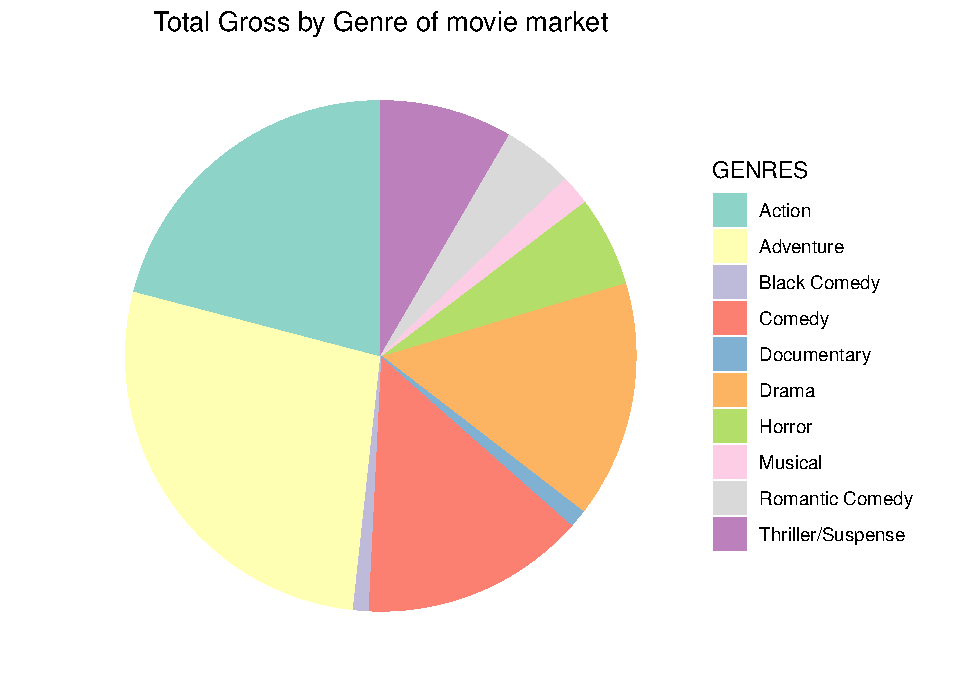
\includegraphics{Final-project_files/figure-latex/unnamed-chunk-1-1.pdf}

In order to find out what kind of movie genres are more popular. I
decided to first check the popularity share of different movie genres in
the market. Therefore pie charts are a good choice for visualization.Pie
charts show how different categories relate to each other as parts of a
whole. Each slice of the pie represents a category, and its Each slice
of the pie represents a category, and its size shows the proportion or
percentage of that category relative to the entire dataset.In order to
have a more visual view of the market share of each movie genre I chose
to use different colors to represent the different genres.Based on the
pie chart, the genre of Adventure have the highest market popularity.
However, genres pf black comedy, documentary, and musical are the less
popular.

\begin{Shaded}
\begin{Highlighting}[]
\CommentTok{\# using ggplot to explore the specific detail of total gross of genres}
\FunctionTok{ggplot}\NormalTok{(TopGenres, }\FunctionTok{aes}\NormalTok{(}\AttributeTok{x =}\NormalTok{ GENRES, }\AttributeTok{y =}\NormalTok{ TOTAL.GROSS)) }\SpecialCharTok{+}
  \FunctionTok{geom\_col}\NormalTok{(}\AttributeTok{width =} \FloatTok{0.5}\NormalTok{, }\AttributeTok{fill =} \StringTok{"skyblue"}\NormalTok{, }\AttributeTok{color =} \StringTok{"black"}\NormalTok{) }\SpecialCharTok{+}  \CommentTok{\# Customize bar appearance}
  \FunctionTok{geom\_segment}\NormalTok{(}\FunctionTok{aes}\NormalTok{(}\AttributeTok{x =}\NormalTok{ GENRES, }\AttributeTok{xend =}\NormalTok{ GENRES, }\AttributeTok{y =} \DecValTok{0}\NormalTok{, }\AttributeTok{yend =}\NormalTok{ TOTAL.GROSS }\SpecialCharTok{+} \DecValTok{5}\NormalTok{),  }\CommentTok{\# Add pin segments}
               \AttributeTok{color =} \StringTok{"black"}\NormalTok{, }\AttributeTok{size =} \DecValTok{1}\NormalTok{) }\SpecialCharTok{+}
  \FunctionTok{geom\_point}\NormalTok{(}\FunctionTok{aes}\NormalTok{(}\AttributeTok{x =}\NormalTok{ GENRES, }\AttributeTok{y =}\NormalTok{ TOTAL.GROSS }\SpecialCharTok{+} \DecValTok{5}\NormalTok{), }\AttributeTok{shape =} \DecValTok{18}\NormalTok{, }\AttributeTok{size =} \FloatTok{2.5}\NormalTok{, }\AttributeTok{color =} \StringTok{"black"}\NormalTok{) }\SpecialCharTok{+}\CommentTok{\# Add pin heads}
  \FunctionTok{labs}\NormalTok{(}\AttributeTok{x =} \StringTok{"}\SpecialCharTok{\textbackslash{}n}\StringTok{Genres Of Movies"}\NormalTok{, }\AttributeTok{y =} \StringTok{"Total Gross Price in billion of dollars"}\NormalTok{, }\AttributeTok{title =} \StringTok{"Bar Graph Of Total Gross Price In Billion Of Dollars by Genres Of Movies"}\NormalTok{) }\SpecialCharTok{+}  \CommentTok{\# Customize labels}
  \FunctionTok{theme}\NormalTok{(}\AttributeTok{axis.text.x =} \FunctionTok{element\_text}\NormalTok{(}\AttributeTok{angle =} \DecValTok{45}\NormalTok{, }\AttributeTok{vjust =} \DecValTok{1}\NormalTok{)) }\SpecialCharTok{+}  \CommentTok{\# Rotate x{-}axis label}
\FunctionTok{scale\_y\_continuous}\NormalTok{(}\AttributeTok{labels =} \ControlFlowTok{function}\NormalTok{(x) }\FunctionTok{format}\NormalTok{(x }\SpecialCharTok{/} \FloatTok{1e9}\NormalTok{, }\AttributeTok{scientific =} \ConstantTok{FALSE}\NormalTok{, }\AttributeTok{big.mark =} \StringTok{","}\NormalTok{, }\AttributeTok{decimal.mark =} \StringTok{"."}\NormalTok{, }\AttributeTok{suffix =} \StringTok{"B"}\NormalTok{)) }\SpecialCharTok{+}
  \FunctionTok{theme\_minimal}\NormalTok{() }\CommentTok{\# Apply a minimal theme}
\end{Highlighting}
\end{Shaded}

\begin{verbatim}
## Warning: Using `size` aesthetic for lines was deprecated in ggplot2 3.4.0.
## i Please use `linewidth` instead.
## This warning is displayed once every 8 hours.
## Call `lifecycle::last_lifecycle_warnings()` to see where this warning was
## generated.
\end{verbatim}

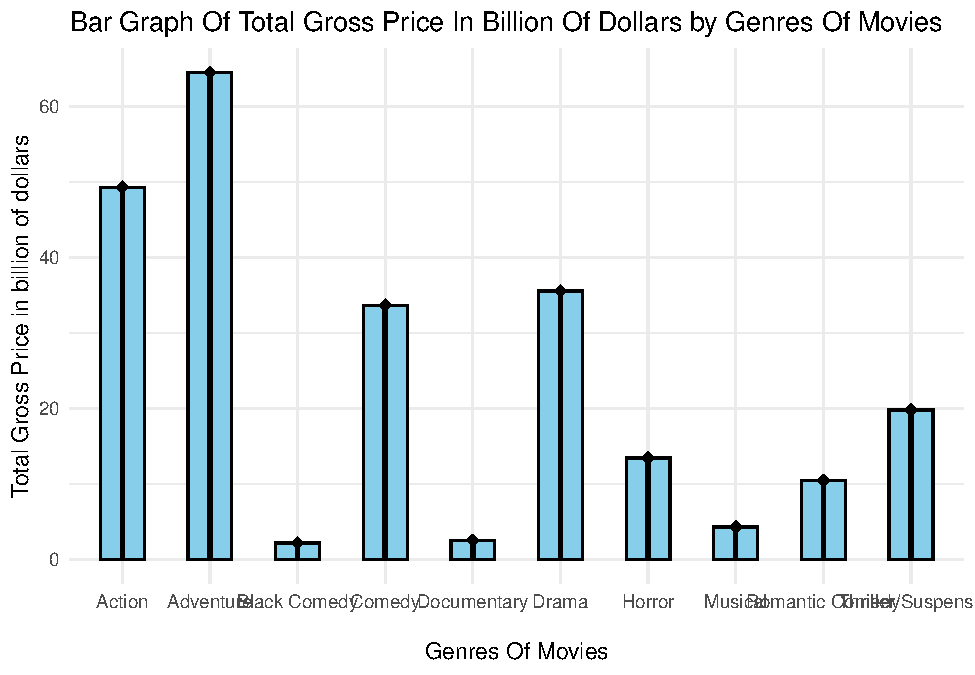
\includegraphics{Final-project_files/figure-latex/unnamed-chunk-2-1.pdf}

However, based on the pie chart could not generate further summary about
the money making based on movie genres. Hence, I create a bar graph
about total gross price in billion of dollars of genres of movies.Bar
graphs are a versatile and commonly used type of chart that help to
visually represent data. They can be very effective for displaying and
comparing information across different categories. To more visually see
the market share of movie genres, I've arranged the bar charts from
largest to smallest and added black lines to better visualize specific
box office amounts. For adventure genres, it has the highest gross at
more than 6000 billion of dollar. Second, is action, it has almost 5000
billion of dollar. Thirdly is drama, it has about 3800 billion of dollar
as total gross.

\hypertarget{research-question-2}{%
\section{Research Question 2}\label{research-question-2}}

\hypertarget{eda---top-distributors}{%
\subsection{EDA - Top Distributors}\label{eda---top-distributors}}

For the second research question, we want to explore the number of
releases of the big six studios and their total gross. Some attributes
we are focusing on are: MOVIES - number of movie release

\begin{Shaded}
\begin{Highlighting}[]
\NormalTok{TopDistributors }\OtherTok{\textless{}{-}}\NormalTok{ TopDistributors[}\SpecialCharTok{{-}}\FunctionTok{c}\NormalTok{(}\DecValTok{7}\NormalTok{,}\DecValTok{8}\NormalTok{,}\DecValTok{9}\NormalTok{,}\DecValTok{10}\NormalTok{),] }\CommentTok{\# delete the rows that will not be focused on for this research}

\CommentTok{\# convert total gross and average gross to integers }
\NormalTok{TopDistributors}\SpecialCharTok{$}\NormalTok{TOTAL.GROSS }\OtherTok{\textless{}{-}}  \FunctionTok{gsub}\NormalTok{(}\StringTok{"}\SpecialCharTok{\textbackslash{}\textbackslash{}}\StringTok{$"}\NormalTok{, }\StringTok{""}\NormalTok{, TopDistributors}\SpecialCharTok{$}\NormalTok{TOTAL.GROSS) }
\NormalTok{TopDistributors}\SpecialCharTok{$}\NormalTok{TOTAL.GROSS }\OtherTok{\textless{}{-}}  \FunctionTok{gsub}\NormalTok{(}\StringTok{","}\NormalTok{, }\StringTok{""}\NormalTok{, TopDistributors}\SpecialCharTok{$}\NormalTok{TOTAL.GROSS) }
\NormalTok{TopDistributors}\SpecialCharTok{$}\NormalTok{TOTAL.GROSS }\OtherTok{\textless{}{-}} \FunctionTok{as.numeric}\NormalTok{(TopDistributors}\SpecialCharTok{$}\NormalTok{TOTAL.GROSS)}
\NormalTok{TopDistributors}\SpecialCharTok{$}\NormalTok{AVERAGE.GROSS }\OtherTok{\textless{}{-}}  \FunctionTok{gsub}\NormalTok{(}\StringTok{"}\SpecialCharTok{\textbackslash{}\textbackslash{}}\StringTok{$"}\NormalTok{, }\StringTok{""}\NormalTok{, TopDistributors}\SpecialCharTok{$}\NormalTok{AVERAGE.GROSS) }
\NormalTok{TopDistributors}\SpecialCharTok{$}\NormalTok{AVERAGE.GROSS }\OtherTok{\textless{}{-}}  \FunctionTok{gsub}\NormalTok{(}\StringTok{","}\NormalTok{, }\StringTok{""}\NormalTok{, TopDistributors}\SpecialCharTok{$}\NormalTok{AVERAGE.GROSS) }
\NormalTok{TopDistributors}\SpecialCharTok{$}\NormalTok{AVERAGE.GROSS }\OtherTok{\textless{}{-}} \FunctionTok{as.numeric}\NormalTok{(TopDistributors}\SpecialCharTok{$}\NormalTok{AVERAGE.GROSS)}

\CommentTok{\# convert the unit of total gross and average gross to billion of dollar and million of dollar}
\NormalTok{TopDistributors }\OtherTok{\textless{}{-}}\NormalTok{ TopDistributors }\SpecialCharTok{\%\textgreater{}\%} 
  \FunctionTok{mutate}\NormalTok{(}\AttributeTok{TOTAL\_GROSS\_in\_Billion =}\NormalTok{ TOTAL.GROSS}\SpecialCharTok{/}\DecValTok{1000000000}\NormalTok{) }\SpecialCharTok{\%\textgreater{}\%} 
  \FunctionTok{mutate}\NormalTok{(}\AttributeTok{AVERAGE\_GROSS\_in\_Million =}\NormalTok{ AVERAGE.GROSS}\SpecialCharTok{/}\DecValTok{1000000}\NormalTok{)}
  

\FunctionTok{ggplot}\NormalTok{(TopDistributors) }\SpecialCharTok{+}
  \FunctionTok{aes}\NormalTok{(}
    \AttributeTok{x =}\NormalTok{ MOVIES,}
    \AttributeTok{y =}\NormalTok{ TOTAL\_GROSS\_in\_Billion,}
    \AttributeTok{colour =}\NormalTok{ DISTRIBUTORS,}
    \AttributeTok{size =}\NormalTok{ AVERAGE\_GROSS\_in\_Million}
\NormalTok{  ) }\SpecialCharTok{+}
  \FunctionTok{geom\_point}\NormalTok{(}\AttributeTok{shape =} \StringTok{"circle"}\NormalTok{) }\SpecialCharTok{+} \CommentTok{\# create the scatter plot where the number of movie is x and the total gross is y, color is the distributors, and size is the average gross}
  \FunctionTok{scale\_color\_hue}\NormalTok{(}\AttributeTok{direction =} \DecValTok{1}\NormalTok{) }\SpecialCharTok{+}
  \FunctionTok{labs}\NormalTok{(}\AttributeTok{title =} \StringTok{"Movie Release vs. Total Gross"}\NormalTok{, }\AttributeTok{color =} \StringTok{"Distributors"}\NormalTok{, }\AttributeTok{size =} \StringTok{"Average Gross in Million of Dollars"}\NormalTok{) }\SpecialCharTok{+} \CommentTok{\# add the title and change the label for x and y axis}
  \FunctionTok{xlab}\NormalTok{(}\StringTok{"}\SpecialCharTok{\textbackslash{}n}\StringTok{Movie"}\NormalTok{) }\SpecialCharTok{+}
  \FunctionTok{ylab}\NormalTok{(}\StringTok{"Total Gross in Billion of Dollars}\SpecialCharTok{\textbackslash{}n}\StringTok{"}\NormalTok{) }\SpecialCharTok{+}
  \FunctionTok{scale\_x\_continuous}\NormalTok{(}\AttributeTok{n.breaks =} \DecValTok{5}\NormalTok{, }\AttributeTok{limits =} \FunctionTok{c}\NormalTok{(}\DecValTok{400}\NormalTok{, }\DecValTok{900}\NormalTok{)) }\SpecialCharTok{+}  \CommentTok{\# change the range scale for x and y axis}
  \FunctionTok{scale\_y\_continuous}\NormalTok{(}\AttributeTok{n.breaks =} \DecValTok{5}\NormalTok{, }\AttributeTok{limits =} \FunctionTok{c}\NormalTok{(}\DecValTok{20}\NormalTok{, }\DecValTok{45}\NormalTok{)) }\SpecialCharTok{+}
  \FunctionTok{scale\_size\_continuous}\NormalTok{(}\AttributeTok{limits =} \FunctionTok{c}\NormalTok{(}\DecValTok{35}\NormalTok{, }\DecValTok{70}\NormalTok{)) }\SpecialCharTok{+}
  \FunctionTok{theme\_light}\NormalTok{() }\SpecialCharTok{+}
  \FunctionTok{guides}\NormalTok{(}\AttributeTok{color =} \FunctionTok{guide\_legend}\NormalTok{(}\AttributeTok{override.aes =} \FunctionTok{list}\NormalTok{(}\AttributeTok{size =} \DecValTok{3}\NormalTok{))) }\SpecialCharTok{+}
  \FunctionTok{theme}\NormalTok{(}
    \AttributeTok{plot.title =} \FunctionTok{element\_text}\NormalTok{(}\AttributeTok{size =}\NormalTok{ 15L,}
    \AttributeTok{face =} \StringTok{"italic"}\NormalTok{,}
    \AttributeTok{hjust =} \FloatTok{0.5}\NormalTok{),}
    \AttributeTok{axis.title.y =} \FunctionTok{element\_text}\NormalTok{(}\AttributeTok{size =}\NormalTok{ 12L),   }\CommentTok{\# change the size of text and legend }
    \AttributeTok{axis.title.x =} \FunctionTok{element\_text}\NormalTok{(}\AttributeTok{size =}\NormalTok{ 12L),}
    \AttributeTok{legend.text =} \FunctionTok{element\_text}\NormalTok{(}\AttributeTok{size =} \DecValTok{10}\NormalTok{), }
    \AttributeTok{legend.title =} \FunctionTok{element\_text}\NormalTok{(}\AttributeTok{size =} \DecValTok{10}\NormalTok{),}
    \AttributeTok{legend.key.height =} \FunctionTok{unit}\NormalTok{(}\FloatTok{0.5}\NormalTok{, }\StringTok{\textquotesingle{}cm\textquotesingle{}}\NormalTok{),}
    \AttributeTok{legend.key.width =} \FunctionTok{unit}\NormalTok{(}\FloatTok{1.5}\NormalTok{, }\StringTok{\textquotesingle{}cm\textquotesingle{}}\NormalTok{)}
\NormalTok{  )}
\end{Highlighting}
\end{Shaded}

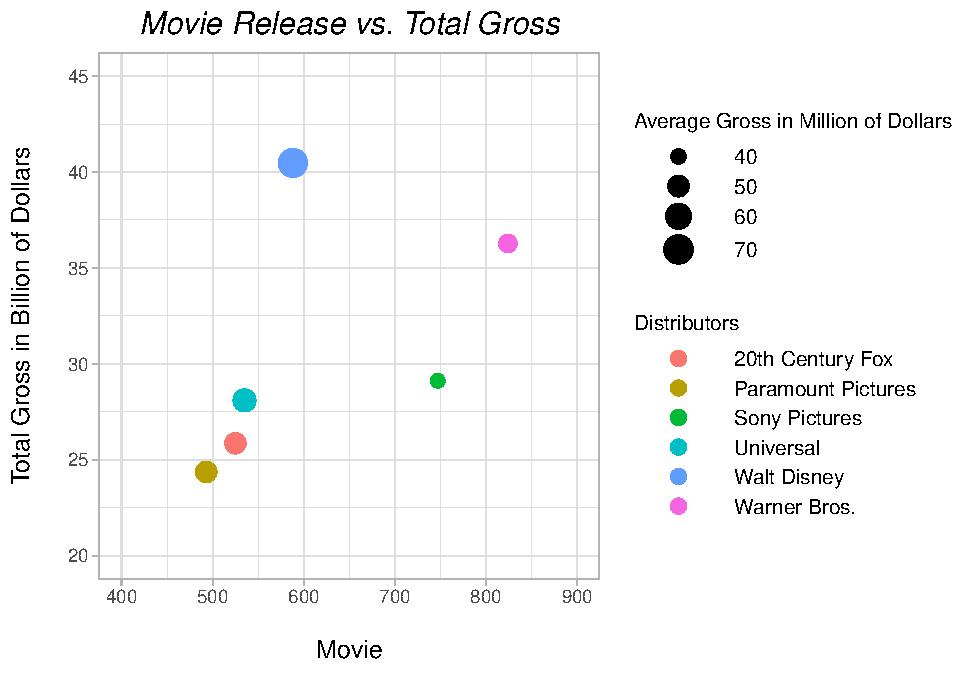
\includegraphics{Final-project_files/figure-latex/unnamed-chunk-3-1.pdf}

\end{document}
